%------------------------------------------------------------------------------
%	DOCUMENT KOMA CLASS
%------------------------------------------------------------------------------

% Remove useless warnings
\RequirePackage{silence} % :-\
    \WarningFilter{scrreprt}{Usage of package `titlesec'}
    \WarningFilter{scrreprt}{Activating an ugly workaround}
    \WarningFilter{titlesec}{Non standard sectioning command detected}

\documentclass[
  % double side thesis
  twoside,openright,
  % primary font size
  fontsize=11pt,
  paper=b5,
  % new page after the title
  titlepage,
  % no point after section number
  numbers=noenddot,
  % header and footer at foot of the page
  headinclude=true,
  footinclude=true,
  % 5 mm bookbinding
  BCOR5mm,
  % empty pages without header at foot of the page
  cleardoublepage=empty,
  abstract=on,
  parskip=half,
  DIV=calc,
  % Languages
  american
]{scrreprt}

%------------------------------------------------------------------------------
%	PACKAGES AND OTHER DOCUMENT CONFIGURATIONS
%------------------------------------------------------------------------------

% so that thesis is printed in an A4 paper and has marks to cut down the paper
% \usepackage[a4,axes,cam,center]{crop}



%------------------------------------------------------------------------------
% 0. Set the encoding of your files. UTF-8 is the only sensible encoding nowadays. If you can't read
% äöüßáéçèê∂åëæƒÏ€ then change the encoding setting in your editor, not the line below. If your editor
% does not support utf8 use another editor!
%------------------------------------------------------------------------------

\PassOptionsToPackage{utf8}{inputenc}
  \usepackage{inputenc}

\PassOptionsToPackage{T1}{fontenc} % T2A for cyrillics
  \usepackage{fontenc}


%------------------------------------------------------------------------------
% 1. Configure classicthesis for your needs here, e.g., remove "drafting" below
% in order to deactivate the time-stamp on the pages
% (see ClassicThesis.pdf for more information):
%------------------------------------------------------------------------------

\PassOptionsToPackage{
  % print version information on the bottom of the pages
  drafting=true,
  % the left column of the toc will be aligned (no indentation)
  tocaligned=false,
  % page numbers in ToC flushed right
  dottedtoc=false,
  % use AMS Euler for chapter font (otherwise Palatino)
  eulerchapternumbers=true,
  % chaper headers will have line above and beneath
  linedheaders=false,
  % numbering per chapter for all floats (i.e., Figure 1.1)
  floatperchapter=true,
  % use awesome Euler fonts for mathematical formulae (only with pdfLaTeX)
  eulermath=false,
  % toggle a nice monospaced font (w/ bold)
  beramono=true,
  % deactivate standard font for loading another one, see the last section at the end of this file for suggestions
  palatino=true,
  style=latex-components/style/classicthesis-arsclassica % classicthesis, arsclassica
}{latex-components/style/classicthesis}


%------------------------------------------------------------------------------
% 2. Personal data and user ad-hoc commands (insert your own data here)
%------------------------------------------------------------------------------

\newcommand{\myTitle}{The structure of pollination networks\xspace}
\newcommand{\mySubtitle}{causes \& consequences\xspace}
\newcommand{\myDegree}{Doctoral thesis\xspace}
\newcommand{\myName}{Fernando Cagua\xspace}
\newcommand{\myProf}{Daniel Stouffer\xspace}
\newcommand{\myOtherProf}{Jason Tylianakis\xspace}
\newcommand{\mySupervisor}{Daniel Stouffer\xspace}
\newcommand{\myFaculty}{College of Science\xspace}
\newcommand{\myDepartment}{School of Biological Sciences\xspace}
\newcommand{\myUni}{University of Canterbury\xspace}
\newcommand{\myLocation}{Christchurch, New Zealand\xspace}
\newcommand{\myTime}{December 2019\xspace}
\newcommand{\myVersion}{Version 0.2}

%------------------------------------------------------------------------------
% Setup, finetuning, and useful commands
%------------------------------------------------------------------------------

\providecommand{\mLyX}{L\kern-.1667em\lower.25em\hbox{Y}\kern-.125emX\@}
\newcommand{\ie}{i.\,e.}
\newcommand{\Ie}{I.\,e.}
\newcommand{\eg}{e.\,g.}
\newcommand{\Eg}{E.\,g.}

%------------------------------------------------------------------------------
% 3. Loading some handy packages
%------------------------------------------------------------------------------


% Packages with options that might require adjustments
%------------------------------------------------------------------------------

% change this to your language(s), main language last
% Spanish languages need extra options in order to work with this template
\PassOptionsToPackage{czech,spanish,es-lcroman,main=british}{babel}
\usepackage{babel}

\usepackage{csquotes}
\PassOptionsToPackage{%
  backend=biber,bibencoding=utf8, %instead of bibtex
  %backend=bibtex8,bibencoding=ascii,%
  language=auto,%
  % style=numeric-comp,%
  style=authoryear, % Author 1999, 2010
  %bibstyle=authoryear,dashed=false, % dashed: substitute rep. author with ---
  sorting=nyt, % name, year, title
  maxbibnames=99, % default: 3, et al.
  % giveninits=true
  %backref=true,%
  % natbib=true % natbib compatibility mode (\citep and \citet still work)
}{biblatex}
\usepackage{biblatex}

% math environments and more by the AMS
\PassOptionsToPackage{fleqn}{amsmath}
\usepackage{amsmath}

% General useful packages
%------------------------------------------------------------------------------

\PassOptionsToPackage{pdftex}{graphicx}
\usepackage{graphicx}
\usepackage{scrhack} % fix warnings when using KOMA with listings package
\usepackage{fixltx2e} % Fixes some LaTeX stuff
\usepackage{xspace} % to get the spacing after macros right
\PassOptionsToPackage{printonlyused,smaller}{acronym}
  \usepackage{acronym} % nice macros for handling all acronyms in the thesis
  %\renewcommand{\bflabel}[1]{{#1}\hfill} % fix the list of acronyms --> no longer working
  %\renewcommand*{\acsfont}[1]{\textsc{#1}}
  %\renewcommand*{\aclabelfont}[1]{\acsfont{#1}}
  %\def\bflabel#1{{#1\hfill}}
  \def\bflabel#1{{\acsfont{#1}\hfill}}
  \def\aclabelfont#1{\acsfont{#1}}
%\usepackage{pgfplots} % External TikZ/PGF support (thanks to Andreas Nautsch)
%\usetikzlibrary{external}
%\tikzexternalize[mode=list and make, prefix=ext-tikz/]

% ornaments
\usepackage{adforn}

%------------------------------------------------------------------------------
% 4. Setup floats: tables, (sub)figures, and captions
%------------------------------------------------------------------------------

% better tables
\usepackage{tabularx}
  % increase table row height
  \setlength{\extrarowheight}{3pt}
\newcommand{\tableheadline}[1]{\multicolumn{1}{l}{\spacedlowsmallcaps{#1}}}
% to be used with each float for alignment
\newcommand{\myfloatalign}{\centering}
\usepackage{caption}
\captionsetup{format=hang,font=small}
\usepackage{subfig}

% SO that floats that are larger than this number get their own page
\renewcommand{\floatpagefraction}{.4}

% so can include float barriers if necessary /FloatBarrier
\usepackage{placeins}

% Packages for kable extra
\usepackage{booktabs}
\usepackage{longtable}
\usepackage{array}
\usepackage{multirow}
\usepackage{wrapfig}
\usepackage{float}
\usepackage{colortbl}
\usepackage{pdflscape}
\usepackage{tabu}
\usepackage{threeparttable}
\usepackage{threeparttablex}
\usepackage[normalem]{ulem}
\usepackage{makecell}
% \usepackage{xcolor} - Dont call xcolor because it's already called by classicthesis

% Using czech in babel breaks booktabs
\usepackage{etoolbox}
\preto\tabular{\shorthandoff{-}}


%------------------------------------------------------------------------------
% 5. Setup code listings
%------------------------------------------------------------------------------

% \usepackage{listings}
% % for special keywords
% %\lstset{emph={trueIndex,root},emphstyle=\color{BlueViolet}}%\underbar}
% \lstset{language=[LaTeX]Tex,%C++,
%   morekeywords={PassOptionsToPackage,selectlanguage},
%   keywordstyle=\color{RoyalBlue},%\bfseries,
%   basicstyle=\small\ttfamily,
%   %identifierstyle=\color{NavyBlue},
%   commentstyle=\color{Green}\ttfamily,
%   stringstyle=\rmfamily,
%   numbers=none,%left,%
%   numberstyle=\scriptsize,%\tiny
%   stepnumber=5,
%   numbersep=8pt,
%   showstringspaces=false,
%   breaklines=true,
%   %frameround=ftff,
%   %frame=single,
%   belowcaptionskip=.75\baselineskip
%   %frame=L
% }

%------------------------------------------------------------------------------
% 6. Last calls before the bar closes
%------------------------------------------------------------------------------

% Her Majesty herself
%------------------------------------------------------------------------------
\usepackage{latex-components/style/classicthesis}
\usepackage{latex-components/style/classicthesis-arsclassica}

%------------------------------------------------------------------------------
% Fine-tune hyperreferences (hyperref should be called last)
%------------------------------------------------------------------------------

\hypersetup{%
  %draft, % hyperref's draft mode, for printing see below
  colorlinks=true, linktocpage=true, pdfstartpage=3, pdfstartview=FitV,%
  % uncomment the following line if you want to have black links (e.g., for printing)
  %colorlinks=false, linktocpage=false, pdfstartpage=3, pdfstartview=FitV, pdfborder={0 0 0},%
  breaklinks=true, pageanchor=true,%
  pdfpagemode=UseNone, %
  % pdfpagemode=UseOutlines,%
  plainpages=false, bookmarksnumbered, bookmarksopen=true, bookmarksopenlevel=1,%
  hypertexnames=true, pdfhighlight=/O,%nesting=true,%frenchlinks,%
  urlcolor=Maroon, linkcolor=Maroon, citecolor=Maroon, pagecolor=Maroon,%
  % urlcolor=Gray, linkcolor=Gray, citecolor=Gray, pagecolor=Gray,%
  pdftitle={\myTitle},%
  pdfauthor={\textcopyright\ \myName, \myUni, \myFaculty},%
  pdfsubject={},%
  pdfkeywords={},%
  pdfcreator={pdfLaTeX},%
  pdfproducer={LaTeX with hyperref and classicthesis}%
}


%------------------------------------------------------------------------------
% Setup autoreferences (hyperref and babel)
%------------------------------------------------------------------------------
% There are some issues regarding autorefnames
% http://www.tex.ac.uk/cgi-bin/texfaq2html?label=latexwords
% you have to redefine the macros for the
% language you use, e.g., american, ngerman
% (as chosen when loading babel/AtBeginDocument)
%------------------------------------------------------------------------------

\makeatletter
\@ifpackageloaded{babel}%
  {%
    \addto\extrasbritish{%
      \renewcommand*{\figureautorefname}{Figure}%
      \renewcommand*{\tableautorefname}{Table}%
      \renewcommand*{\partautorefname}{Part}%
      \renewcommand*{\chapterautorefname}{Chapter}%
      \renewcommand*{\sectionautorefname}{Section}%
      \renewcommand*{\subsectionautorefname}{Section}%
      \renewcommand*{\subsubsectionautorefname}{Section}%
    }%
    \addto\extrasngerman{%
      \renewcommand*{\paragraphautorefname}{Absatz}%
      \renewcommand*{\subparagraphautorefname}{Unterabsatz}%
      \renewcommand*{\footnoteautorefname}{Fu\"snote}%
      \renewcommand*{\FancyVerbLineautorefname}{Zeile}%
      \renewcommand*{\theoremautorefname}{Theorem}%
      \renewcommand*{\appendixautorefname}{Anhang}%
      \renewcommand*{\equationautorefname}{Gleichung}%
      \renewcommand*{\itemautorefname}{Punkt}%
    }%
      % Fix to getting autorefs for subfigures right (thanks to Belinda Vogt for changing the definition)
      \providecommand{\subfigureautorefname}{\figureautorefname}%
    }{\relax}
\makeatother


% Backreferences

% \usepackage{ifthen} % Allows the user of the \ifthenelse command
% \newboolean{enable-backrefs} % Variable to enable backrefs in the bibliography
% \setboolean{enable-backrefs}{false} % Variable value: true or false
%
% \newcommand{\backrefnotcitedstring}{\relax} % (Not cited.)
% \newcommand{\backrefcitedsinglestring}[1]{(Cited on page~#1.)}
% \newcommand{\backrefcitedmultistring}[1]{(Cited on pages~#1.)}
% \ifthenelse{\boolean{enable-backrefs}} % If backrefs were enabled
% {
% \PassOptionsToPackage{hyperpageref}{backref}
% \usepackage{backref} % to be loaded after hyperref package
% \renewcommand{\backreftwosep}{ and~} % separate 2 pages
% \renewcommand{\backreflastsep}{, and~} % separate last of longer list
% \renewcommand*{\backref}[1]{}  % disable standard
% \renewcommand*{\backrefalt}[4]{% detailed backref
% \ifcase #1
% \backrefnotcitedstring
% \or
% \backrefcitedsinglestring{#2}
% \else
% \backrefcitedmultistring{#2}
% \fi}
% }{\relax}

%------------------------------------------------------------------------------
% Development Stuff
%------------------------------------------------------------------------------
\listfiles
%\PassOptionsToPackage{l2tabu,orthodox,abort}{nag}
%  \usepackage{nag}
%\PassOptionsToPackage{warning, all}{onlyamsmath}
%  \usepackage{onlyamsmath}


%------------------------------------------------------------------------------
% 7. Further adjustments (experimental)
%------------------------------------------------------------------------------

% Changing the text area
%------------------------------------------------------------------------------
%\areaset[current]{312pt}{761pt} % 686 (factor 2.2) + 33 head + 42 head \the\footskip
%\setlength{\marginparwidth}{7em}%
%\setlength{\marginparsep}{2em}%

% Using different fonts
%------------------------------------------------------------------------------

%\usepackage[oldstylenums]{kpfonts} % oldstyle notextcomp
% \usepackage[osf]{libertine}
%\usepackage[light,condensed,math]{iwona}
%\renewcommand{\sfdefault}{iwona}
%\usepackage{lmodern} % <-- no osf support :-(
%\usepackage{cfr-lm} %
%\usepackage[urw-garamond]{mathdesign} <-- no osf support :-(
%\usepackage[default,osfigures]{opensans} % scale=0.95
%\usepackage[sfdefault]{FiraSans}
% \usepackage[opticals,mathlf]{MinionPro} % onlytext

%\usepackage[largesc,osf]{newpxtext}
%\linespread{1.05} % a bit more for Palatino
% Used to fix these:
% https://bitbucket.org/amiede/classicthesis/issues/139/italics-in-pallatino-capitals-chapter
% https://bitbucket.org/amiede/classicthesis/issues/45/problema-testatine-su-classicthesis-style

% Glossary and acronyms
\usepackage[style=index,nolist,toc]{glossaries}
\makenoidxglossaries

\newglossaryentry{network control}{
  name={network control},
  description={a network is said to be controllable if it is possible to steer it from an initial to an arbitrary final state within finite time}}

\newglossaryentry{controllability}{
  name={controllability},
  description={the intrinsic difficulty of controlling an ecological community. It is measured by the relative size of the minimum driver-node set, $n_D$. It also indicates the extent to which network structure can be harnessed for network control}}

\newglossaryentry{minimum driver node set}{
  name={minimum driver-node set},
  description={one of the sets of species whose abundances need to be directly managed in order to achieve full control of the community. The minimum driver-node sets can be obtained by finding all maximum matchings in a network}}

\newglossaryentry{maximum matching}{
  name={maximum matching},
  description={a matching is a set of links that do not share any common start or end nodes; the largest possible matching is called a maximum matching}}

\newglossaryentry{control configuration}{
  name={control configuration},
  description={one of the species combinations with which is possible to achieve network control. Optimal control configurations are given by the minimum driver-node sets}}

\newglossaryentry{control capacity}{
  name={control capacity},
  description={the relative frequency ($\phi$) which with a species is part of the optimal control configurations of a network}}

\newglossaryentry{critical species}{
  name={critical species},
  description={a species with a maximal control capacity ($\phi=1$)}}

\newglossaryentry{superior node}{
  name={superior node},
  description={a species is a superior node if it can internally affect the abundance of other species in the network. Superior nodes make up the chains that propagate the control signals through the network}}


% add declaration from an external file

\usepackage{pdfpages}

%------------------------------------------------------------------------------
% BIBLIOGRAPHY
%------------------------------------------------------------------------------

\addbibresource{bibliography/phd-literature.bib}

\DeclareSourcemap{
  \maps[datatype=bibtex]{
    \map{
      \step[fieldset=issn, null]
      \step[fieldset=editor, null]
    }
  }
}

% \fullcite to show all authors
\preto\fullcite{\AtNextCite{\defcounter{maxnames}{99}}}

%------------------------------------------------------------------------------
% MAIN DOCUMENT
%------------------------------------------------------------------------------

\begin{document}

\pagenumbering{roman}

%------------------------------------------------------------------------------% % Title page
%------------------------------------------------------------------------------

\begin{titlepage}
    %\pdfbookmark[1]{\myTitle}{titlepage}
    % if you want the titlepage to be centered, uncomment and fine-tune the line below (KOMA classes environment)
    \begin{addmargin}[-1cm]{-3cm}
    \begin{center}
        \large

        \hfill
        \vfill

        \begingroup
        \huge
            \color{CTtitle}\spacedallcaps{\myTitle} \\ \bigskip
        \endgroup

        \begingroup
          \Large
          \textit{\mySubtitle}
        \endgroup


        \bigskip
        \bigskip
        \bigskip

        \begingroup
        \huge
        \adforn{21}
        \endgroup

        \bigskip
        \bigskip
        \bigskip

        \begingroup
        \Large
        \spacedlowsmallcaps{\myName} \\ \medskip
        \endgroup
        \myTime\ -- \myVersion

        \bigskip
        \bigskip
        \bigskip
        \bigskip
        \bigskip

        \begingroup
        \normalsize
        \myDegree \\
        \myDepartment \\
        % \myFaculty \\
        \myUni \\
        \endgroup


        \vfill

    \end{center}
  \end{addmargin}
\end{titlepage}

%------------------------------------------------------------------------------% % Title back
%------------------------------------------------------------------------------

\thispagestyle{empty}

\hfill

\vfill

\noindent\myName: \textit{\myTitle:} \mySubtitle; \myDegree,
\textcopyright\ \myTime

\bigskip
%
\noindent\spacedlowsmallcaps{Supervisors}: \\
\myProf \\
\myOtherProf %\\
% \mySupervisor
%
\medskip

%\noindent\spacedlowsmallcaps{Location}: \\
\myLocation

%\medskip

%\noindent\spacedlowsmallcaps{Date}: \\
%\myTime


\cleardoublepage%------------------------------------------------------------------------------% % Dedication
%------------------------------------------------------------------------------

\thispagestyle{empty}
\phantomsection
\pdfbookmark[1]{Dedication}{Dedication}

\vspace*{3cm}

\begin{center}
    Con amor, en memoria de Betty Helena Bermudez. \\ \smallskip
    1964\,--\,2009
\end{center}


\cleardoublepage%------------------------------------------------------------------------------
% Table of Contents
%------------------------------------------------------------------------------

\pagestyle{scrheadings}
\phantomsection
\pdfbookmark[1]{\contentsname}{tableofcontents}
% \addcontentsline{toc}{chapter}{TOC}
\setcounter{tocdepth}{0} % <-- 2 includes up to subsections in the ToC
\setcounter{secnumdepth}{3} % <-- 3 numbers up to subsubsections
\manualmark
\markboth{\spacedlowsmallcaps{\contentsname}}{\spacedlowsmallcaps{\contentsname}}
\tableofcontents
\automark[section]{chapter}
\renewcommand{\chaptermark}[1]{\markboth{\spacedlowsmallcaps{#1}}{\spacedlowsmallcaps{#1}}}
\renewcommand{\sectionmark}[1]{\markright{\textsc{\thesection}\enspace\spacedlowsmallcaps{#1}}}


% \cleardoublepage%------------------------------------------------------------------------------
% Summary
%------------------------------------------------------------------------------


% English
%------------------------------------------------------------------------------

\phantomsection
\addcontentsline{toc}{chapter}{Summary}
\renewcommand{\abstractname}{Summary}
% \pdfbookmark[1]{Abstract}{Abstract}
% \begingroup
% \let\clearpage\relax
% \let\cleardoublepage\relax
% \let\cleardoublepage\relax

\chapter*{Summary}

\vfill



% \cleardoublepage% Español
%------------------------------------------------------------------------------

\begin{otherlanguage}{spanish}
% \pdfbookmark[1]{Resumen}{Resumen}
\phantomsection
\addcontentsline{toc}{chapter}{Resumen}
\chapter*{Resumen}
Kurze Zusammenfassung des Inhaltes in deutscher Sprache\dots
\end{otherlanguage}

% \endgroup

\vfill

\cleardoublepage%------------------------------------------------------------------------------
% PUBLICATIONS
%------------------------------------------------------------------------------

\phantomsection
\addcontentsline{toc}{chapter}{Publications}
% \setcounter{secnumdepth}{-1}
\chapter*{Publications}
% \setcounter{secnumdepth}{3}

% Hack to get the header right. No idea why it doesn't work properly
\manualmark
\markboth{\spacedlowsmallcaps{Publications}}{\spacedlowsmallcaps{Publications}}
\automark[section]{chapter}

\noindent The following peer-reviewed publications have been published by the candidate during the PhD term.
%
\begin{refsection}
    % \small
    \nocite{*} % is local to to the enclosing refsection
    \printbibliography[heading=none,keyword=own]
\end{refsection}


\vfill

% \cleardoublepage%------------------------------------------------------------------------------
% Declaration
%------------------------------------------------------------------------------

% \pdfbookmark[0]{Coauthorship declaration}{declaration}
% \setcounter{secnumdepth}{-1}
\phantomsection
\addcontentsline{toc}{chapter}{Declaration}
\chapter*{Coauthorship declaration}
\thispagestyle{empty}
% \setcounter{secnumdepth}{3}

\begin{refsection}

% \printbibliography[heading=none]
All chapters in this dissertation have been extracted from co-authored work.

\autoref{pollen-competition} and \autoref{sdm-networks} have been published as a pre-print in \emph{bioRxiv}.
For \autoref{pollen-competition} (p. 865279; \textsc{doi}: \href{https://doi.org/10.1101/865279}{\texttt{10.1101/865279}}) the candidate analysed all data (100\%) and wrote the manuscript's first draft (100\%).
For \autoref{sdm-networks} (p. 866772; \textsc{doi}: \href{https://doi.org/10.1101/866772}{\texttt{10.1101/866772}}) the candidate analysed all data (100\%), wrote the manuscript's first draft (100\%), and contributed to data collection (20\%) and data cleaning (80\%).

\autoref{structural-controllability} has been published in \emph{Journal of Ecology} (107.4, pp. 1365--2745 \textsc{doi}: \href{https://doi.org/10.1111/1365-2745.13147}{\texttt{10.1111/1365-2745.13147}}). The candidate analysed all data (100\%), wrote the the manuscript's first draft (100\%), and contributed to the development of the theoretical framework (80\%).

Finally, \autoref{cophylogeny} has been published in \emph{Ecology} (98.10, pp. 2640--2652; \textsc{doi}: \href{https://doi.org/10.1002/ecy.1955}{\texttt{10.1002/ecy.1955}}). The candidate contributed to data analysis (60\%), manuscript writing (40\%), and data visualisation (70\%).

\end{refsection}

On behalf of all co-authors, the undersigned certifys that: the above statement correctly reflects the nature and extent of the PhD candidate's contribution to this co-authored work; and in cases where the candidate was the lead author of the co-authored work he wrote the text.

\bigskip

\noindent\textit{\myLocation, \myTime}

\smallskip

\begin{flushright}
    \begin{tabular}{m{5cm}}
        \\ \hline
        \centering Daniel B. Stouffer \\
    \end{tabular}
\end{flushright}

\cleardoublepage\phantomsection
\addcontentsline{toc}{chapter}{Declaration}

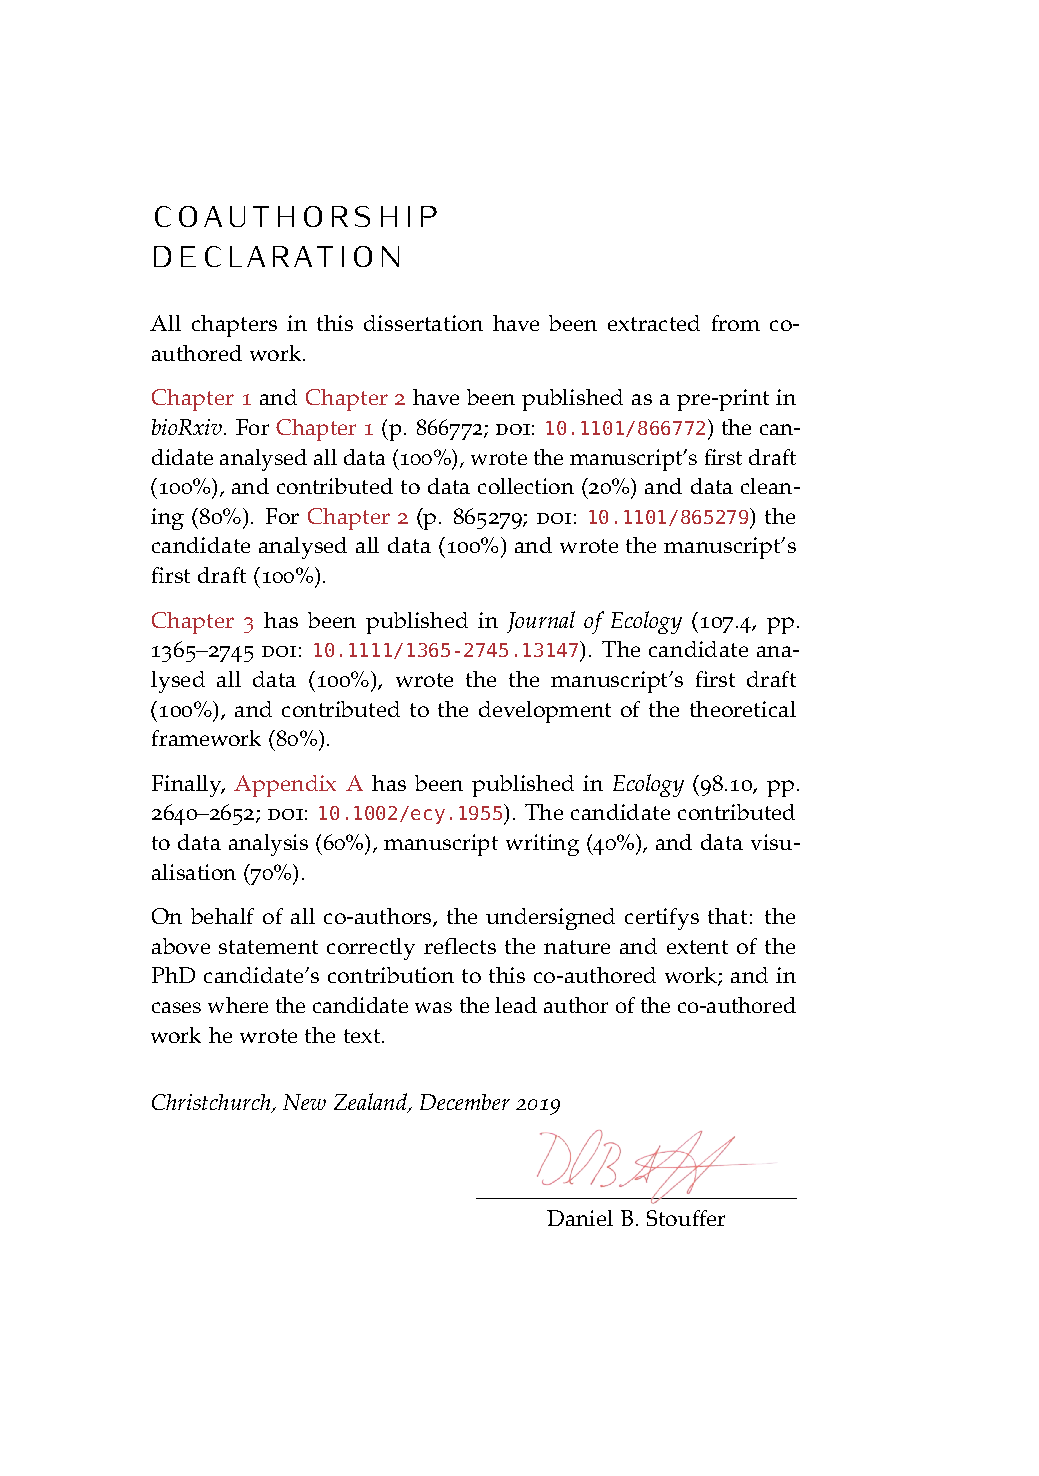
\includepdf{latex-components/front-back-matter/coauthorship-form-signed}

\cleardoublepage\phantomsection
\addcontentsline{toc}{chapter}{Acknowledgments}
\chapter*{Acknowledgments}

\begin{otherlanguage}{spanish}
Gracias a mi familia porque sin ellos no estaría aquí.
En especial a mis hermanitos a los que siempre admiro y extraño.
\end{otherlanguage}
\begin{otherlanguage}{spanish}
Děkuji Petrovi za to, že mi dal pevné zázemí a křídla.
\end{otherlanguage}
\begin{otherlanguage}{spanish}
A Bernat por siempre estar ahí en las buenas y malas.
\end{otherlanguage}

Thanks to Daniel for always encouraging me to give my best.
To Jason for providing safe spaces where ideas can grow.
To both of them for their guidance and advice, I feel lucky to have them both.
Thanks to present and past members of the Stouffer and Tylianakis lab; it was an honour to be in the same team.

To all of those with which we smiled together over the last five years, you all make New Zealand feel home.

\begin{flushright}{\slshape
    We have seen that computer programming is an art, \\
    because it applies accumulated knowledge to the world, \\
    because it requires skill and ingenuity, and especially \\
    because it produces objects of beauty.} \\ \medskip
    % --- \defcitealias{knuth:1974}{Donald E. Knuth}\citetalias{knuth:1974} \citep{knuth:1974}
\end{flushright}

\cleardoublepage%------------------------------------------------------------------------------
% REFACE
%------------------------------------------------------------------------------

\phantomsection
\addcontentsline{toc}{chapter}{Preface}
% \setcounter{secnumdepth}{-1}
\chapter*{Preface}
% \setcounter{secnumdepth}{3}

% Hack to get the header right. No idea why it doesn't work properly
\manualmark
\markboth{\spacedlowsmallcaps{Preface}}{\spacedlowsmallcaps{Preface}}
\automark[section]{chapter}

\noindent This thesis is composed of three scientific articles.
All of these articles study the processes that influence the structure of pollination networks and their implications.
Each chapter is a standalone piece of research and, therefore, I only provide a brief general Introduction and Conclusion linking chapters together.
In the Introduction, I focus on describing the joint context from which the research questions tackled in each chapter originate.
In the Conclusion, I focus on the relationship between each chapter's results and discuss the implications of this relationship for our understanding of pollination networks.

In \autoref{cophylogeny} I include another article that, although it did not end up being an integral part my thesis, it represented an important outcome provided an opportunity to learn and practice essential skills for a successful PhD and eventually led me to the topic of this dissertation.

\vfill

\cleardoublepage\thispagestyle{empty}

\begin{addmargin}[0cm]{-2cm}
  \begin{center}
      \begingroup
      \Large
      \color{CTtitle}\spacedallcaps{\myTitle} \\ \bigskip
    \endgroup
  \end{center}
\end{addmargin}


\newpage
\cleardoublepage
\pagenumbering{arabic}

% Place front matter stuff slightly above the rest of the document content in the table of contents
% \addtocontents{toc}{\protect\vspace{1em}}

$body$

\cleardoublepage%********************************************************************
% Bibliography
%*******************************************************
% work-around to have small caps also here in the headline
% https://tex.stackexchange.com/questions/188126/wrong-header-in-bibliography-classicthesis
% Thanks to Enrico Gregorio
\defbibheading{bibintoc}[\bibname]{%
  \phantomsection
  \manualmark
  \markboth{\spacedlowsmallcaps{#1}}{\spacedlowsmallcaps{#1}}%
  % Place the bibliography slightly below the rest of the document content in the table of contents
  \addtocontents{toc}{\protect\vspace{\beforebibskip}}%
  \addcontentsline{toc}{chapter}{\tocEntry{#1}}%
  \chapter*{#1}%
}
\printbibliography[heading=bibintoc]


% % Bibliography
% %
% \addtocontents{toc}{\protect\vspace{\beforebibskip}} % Place the bibliography slightly below the rest of the document content in the table of contents
% \addcontentsline{toc}{chapter}{\tocEntry{\bibname}}
% \printbibliography[
% heading=bibintoc
% ]
%
% \label{app:bibliography} % Reference the bibliography elsewhere with \autoref{app:bibliography}
% %
% \manualmark
% \markboth{\spacedlowsmallcaps{\bibname}}{\spacedlowsmallcaps{\bibname}}
% \refstepcounter{dummy}
% %

\cleardoublepage%------------------------------------------------------------------------------
% List of Figures and of the Tables
%------------------------------------------------------------------------------

% \pagestyle{empty} % Uncomment this line if your lists should not have any headlines with section name and page number
% \begingroup
    % \let\clearpage\relax
    % \let\cleardoublepage\relax

% List of Figures
%------------------------------------------------------------------------------
    \phantomsection
    \addcontentsline{toc}{chapter}{\listfigurename}
    % \pdfbookmark[1]{\listfigurename}{lof}
    \listoffigures

    \begin{flushright}{\slshape
    Storytellers of all stripes must regularly compress all of the possible information their stories could contain into a manageable number of relatable details } \\ \medskip
    --- Micahel Austin
\end{flushright}

\begin{flushright}{\slshape
    The sole aim of a methaphor is to call up a visual image} \\ \medskip
    --- George Orwell 1946
\end{flushright}

    % \vspace{8ex}
\cleardoublepage

% List of Tables
%------------------------------------------------------------------------------
    \phantomsection
    \addcontentsline{toc}{chapter}{\listtablename}
    % \pdfbookmark[1]{\listtablename}{lot}
    \listoftables

    % \vspace{8ex}
    % \newpage

    % %*******************************************************
    % % List of Listings
    % %*******************************************************
    % %\phantomsection
    % %\addcontentsline{toc}{chapter}{\lstlistlistingname}
    % \pdfbookmark[1]{\lstlistlistingname}{lol}
    % \lstlistoflistings
    %
    % \vspace{8ex}
    %
    % %*******************************************************
    % % Acronyms
    % %*******************************************************
    % %\phantomsection
    % \pdfbookmark[1]{Acronyms}{acronyms}
    % \markboth{\spacedlowsmallcaps{Acronyms}}{\spacedlowsmallcaps{Acronyms}}
    % \chapter*{Acronyms}
    % \begin{acronym}[UMLX]
    %     \acro{DRY}{Don't Repeat Yourself}
    %     \acro{API}{Application Programming Interface}
    %     \acro{UML}{Unified Modeling Language}
    % \end{acronym}

% \endgroup

% \cleardoublepage% \phantomsection
% \addcontentsline{toc}{chapter}{Glossary}
% % \setcounter{secnumdepth}{-1}
% \chapter*{Glossary}

\printnoidxglossary[sort=use]

\cleardoublepage%*******************************************************
% Colophon
%*******************************************************
\cleardoublepage
\pagestyle{empty}

\hfill

\vfill


\pdfbookmark[0]{Colophon}{colophon}
\section*{Colophon}
This document was compiled using the R package \texttt{bookdown} \autocites{bookdown_package}{bookdown_book}. It was typeset using the typographical look-and-feel \texttt{classicthesis} developed by Andr\'e Miede and Ivo Pletikosić for \LaTeX. All text and code can be found in:
\begin{center}
\url{https://github.com/efcaguab/phd-thesis}
\end{center}
Feedback and comments can be directed to:
\begin{center}
\url{fernando@cagua.co}
\end{center}
Thank you.

\bigskip

\noindent\finalVersionString


\end{document}
